% Options for packages loaded elsewhere
\PassOptionsToPackage{unicode}{hyperref}
\PassOptionsToPackage{hyphens}{url}
%
\documentclass[
]{article}
\usepackage{amsmath,amssymb}
\usepackage{iftex}
\ifPDFTeX
  \usepackage[T1]{fontenc}
  \usepackage[utf8]{inputenc}
  \usepackage{textcomp} % provide euro and other symbols
\else % if luatex or xetex
  \usepackage{unicode-math} % this also loads fontspec
  \defaultfontfeatures{Scale=MatchLowercase}
  \defaultfontfeatures[\rmfamily]{Ligatures=TeX,Scale=1}
\fi
\usepackage{lmodern}
\ifPDFTeX\else
  % xetex/luatex font selection
\fi
% Use upquote if available, for straight quotes in verbatim environments
\IfFileExists{upquote.sty}{\usepackage{upquote}}{}
\IfFileExists{microtype.sty}{% use microtype if available
  \usepackage[]{microtype}
  \UseMicrotypeSet[protrusion]{basicmath} % disable protrusion for tt fonts
}{}
\makeatletter
\@ifundefined{KOMAClassName}{% if non-KOMA class
  \IfFileExists{parskip.sty}{%
    \usepackage{parskip}
  }{% else
    \setlength{\parindent}{0pt}
    \setlength{\parskip}{6pt plus 2pt minus 1pt}}
}{% if KOMA class
  \KOMAoptions{parskip=half}}
\makeatother
\usepackage{xcolor}
\usepackage[margin=1in]{geometry}
\usepackage{color}
\usepackage{fancyvrb}
\newcommand{\VerbBar}{|}
\newcommand{\VERB}{\Verb[commandchars=\\\{\}]}
\DefineVerbatimEnvironment{Highlighting}{Verbatim}{commandchars=\\\{\}}
% Add ',fontsize=\small' for more characters per line
\usepackage{framed}
\definecolor{shadecolor}{RGB}{248,248,248}
\newenvironment{Shaded}{\begin{snugshade}}{\end{snugshade}}
\newcommand{\AlertTok}[1]{\textcolor[rgb]{0.94,0.16,0.16}{#1}}
\newcommand{\AnnotationTok}[1]{\textcolor[rgb]{0.56,0.35,0.01}{\textbf{\textit{#1}}}}
\newcommand{\AttributeTok}[1]{\textcolor[rgb]{0.13,0.29,0.53}{#1}}
\newcommand{\BaseNTok}[1]{\textcolor[rgb]{0.00,0.00,0.81}{#1}}
\newcommand{\BuiltInTok}[1]{#1}
\newcommand{\CharTok}[1]{\textcolor[rgb]{0.31,0.60,0.02}{#1}}
\newcommand{\CommentTok}[1]{\textcolor[rgb]{0.56,0.35,0.01}{\textit{#1}}}
\newcommand{\CommentVarTok}[1]{\textcolor[rgb]{0.56,0.35,0.01}{\textbf{\textit{#1}}}}
\newcommand{\ConstantTok}[1]{\textcolor[rgb]{0.56,0.35,0.01}{#1}}
\newcommand{\ControlFlowTok}[1]{\textcolor[rgb]{0.13,0.29,0.53}{\textbf{#1}}}
\newcommand{\DataTypeTok}[1]{\textcolor[rgb]{0.13,0.29,0.53}{#1}}
\newcommand{\DecValTok}[1]{\textcolor[rgb]{0.00,0.00,0.81}{#1}}
\newcommand{\DocumentationTok}[1]{\textcolor[rgb]{0.56,0.35,0.01}{\textbf{\textit{#1}}}}
\newcommand{\ErrorTok}[1]{\textcolor[rgb]{0.64,0.00,0.00}{\textbf{#1}}}
\newcommand{\ExtensionTok}[1]{#1}
\newcommand{\FloatTok}[1]{\textcolor[rgb]{0.00,0.00,0.81}{#1}}
\newcommand{\FunctionTok}[1]{\textcolor[rgb]{0.13,0.29,0.53}{\textbf{#1}}}
\newcommand{\ImportTok}[1]{#1}
\newcommand{\InformationTok}[1]{\textcolor[rgb]{0.56,0.35,0.01}{\textbf{\textit{#1}}}}
\newcommand{\KeywordTok}[1]{\textcolor[rgb]{0.13,0.29,0.53}{\textbf{#1}}}
\newcommand{\NormalTok}[1]{#1}
\newcommand{\OperatorTok}[1]{\textcolor[rgb]{0.81,0.36,0.00}{\textbf{#1}}}
\newcommand{\OtherTok}[1]{\textcolor[rgb]{0.56,0.35,0.01}{#1}}
\newcommand{\PreprocessorTok}[1]{\textcolor[rgb]{0.56,0.35,0.01}{\textit{#1}}}
\newcommand{\RegionMarkerTok}[1]{#1}
\newcommand{\SpecialCharTok}[1]{\textcolor[rgb]{0.81,0.36,0.00}{\textbf{#1}}}
\newcommand{\SpecialStringTok}[1]{\textcolor[rgb]{0.31,0.60,0.02}{#1}}
\newcommand{\StringTok}[1]{\textcolor[rgb]{0.31,0.60,0.02}{#1}}
\newcommand{\VariableTok}[1]{\textcolor[rgb]{0.00,0.00,0.00}{#1}}
\newcommand{\VerbatimStringTok}[1]{\textcolor[rgb]{0.31,0.60,0.02}{#1}}
\newcommand{\WarningTok}[1]{\textcolor[rgb]{0.56,0.35,0.01}{\textbf{\textit{#1}}}}
\usepackage{longtable,booktabs,array}
\usepackage{calc} % for calculating minipage widths
% Correct order of tables after \paragraph or \subparagraph
\usepackage{etoolbox}
\makeatletter
\patchcmd\longtable{\par}{\if@noskipsec\mbox{}\fi\par}{}{}
\makeatother
% Allow footnotes in longtable head/foot
\IfFileExists{footnotehyper.sty}{\usepackage{footnotehyper}}{\usepackage{footnote}}
\makesavenoteenv{longtable}
\usepackage{graphicx}
\makeatletter
\def\maxwidth{\ifdim\Gin@nat@width>\linewidth\linewidth\else\Gin@nat@width\fi}
\def\maxheight{\ifdim\Gin@nat@height>\textheight\textheight\else\Gin@nat@height\fi}
\makeatother
% Scale images if necessary, so that they will not overflow the page
% margins by default, and it is still possible to overwrite the defaults
% using explicit options in \includegraphics[width, height, ...]{}
\setkeys{Gin}{width=\maxwidth,height=\maxheight,keepaspectratio}
% Set default figure placement to htbp
\makeatletter
\def\fps@figure{htbp}
\makeatother
\setlength{\emergencystretch}{3em} % prevent overfull lines
\providecommand{\tightlist}{%
  \setlength{\itemsep}{0pt}\setlength{\parskip}{0pt}}
\setcounter{secnumdepth}{-\maxdimen} % remove section numbering
\ifLuaTeX
  \usepackage{selnolig}  % disable illegal ligatures
\fi
\usepackage{bookmark}
\IfFileExists{xurl.sty}{\usepackage{xurl}}{} % add URL line breaks if available
\urlstyle{same}
\hypersetup{
  pdftitle={Progress report - species validation with Shiny App},
  pdfauthor={Sunny Tseng},
  hidelinks,
  pdfcreator={LaTeX via pandoc}}

\title{Progress report - species validation with Shiny App}
\author{Sunny Tseng}
\date{2024-11-18}

\begin{document}
\maketitle

\subsubsection{Quick review}\label{quick-review}

All validation datasets are stored in a
\href{https://drive.google.com/drive/folders/1-oZjQ5xzwJOD9E9hcm_CSMku05FS9gKa?usp=sharing}{Google
Drive}, organized by species in individual folders. There are 27 target
species, although White-winged Scoter has no detections, so there are
only 26 folders. Each species folder includes up to 180 recording
segments (each 9 seconds long) and a .csv file named ``SPECIES
NAME\_validation.csv'' that serves as metadata for these segments. The
segments are randomly selected from all detections for that species,
stratified by confidence score. The validation task involves listening
to each segment to verify if BirdNET correctly identified the species
and writing down this information in the .csv file. To conduct species
validation, follow these steps:

\subsubsection{Mark species}\label{mark-species}

\begin{itemize}
\item
  In the Google Drive main folder, open the
  ``who\_did\_species\_validation'' file and add your name to indicate
  that you are validating a species (e.g., put my name down beside
  Sora).

  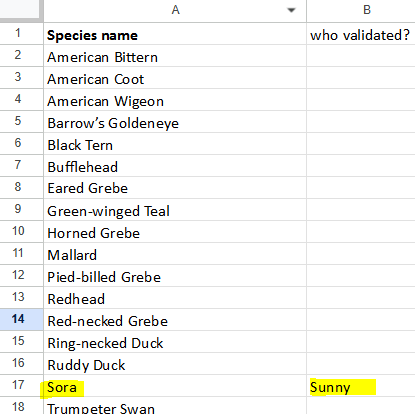
\includegraphics{images/clipboard-1502569650.png}
\end{itemize}

\subsubsection{Get data folder}\label{get-data-folder}

\begin{itemize}
\tightlist
\item
  Download the whole folder for the species that you selected
\end{itemize}

\begin{itemize}
\item
  In the selected species folder, open the ``SPECIES
  NAME\_validation.csv'' file. Add two new columns beside the category
  column labeled ``validation'' and ``note.''

  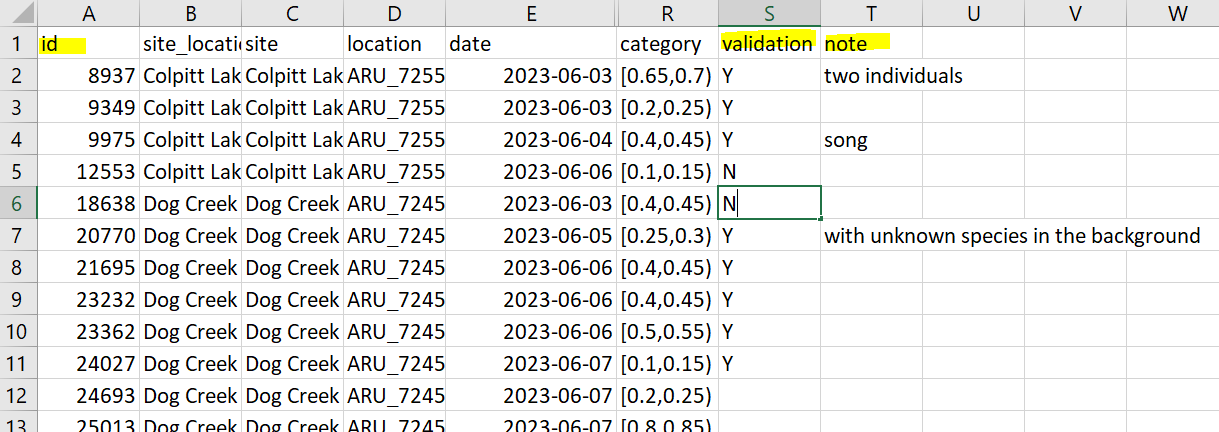
\includegraphics{images/clipboard-1183498283.png}
\end{itemize}

\begin{itemize}
\tightlist
\item
  Listen to each recording and view the spectrogram if needed. If the
  BirdNET detection is accurate (e.g., Sora is present in the
  recording), enter ``Y'' in the validation column. If it is not
  accurate (e.g., no Sora was heard), enter ``N.''
\item
  Record notes on specific vocalizations (e.g., song, call, begging
  call) and/or possible reasons for misidentification (e.g., background
  noise, misidentified as XYZ species).
\item
  To avoid judgement bias, ``hide'' the confidence column by
  \texttt{right\ click\ \textgreater{}\ Hide}.
\end{itemize}

\subsubsection{Use ShinyR to listen/view spectrogram
(optional)}\label{use-shinyr-to-listenview-spectrogram-optional}

\begin{itemize}
\tightlist
\item
  Open RStudio, enter the following chunk of code.
\end{itemize}

\begin{Shaded}
\begin{Highlighting}[]
\CommentTok{\# use install.packages("PACKAGE\_NAME") if you don\textquotesingle{}t have any of the following required package}

\FunctionTok{library}\NormalTok{(shiny) }
\FunctionTok{library}\NormalTok{(bslib)}
\FunctionTok{library}\NormalTok{(shinyWidgets) }
\FunctionTok{library}\NormalTok{(shinyFiles)}

\FunctionTok{library}\NormalTok{(tidyverse)}
\FunctionTok{library}\NormalTok{(DT)}
\FunctionTok{library}\NormalTok{(praise)}

\FunctionTok{library}\NormalTok{(tuneR)}
\FunctionTok{library}\NormalTok{(seewave)}

\NormalTok{shiny}\SpecialCharTok{::}\FunctionTok{runGitHub}\NormalTok{(}\StringTok{"Birds{-}Canada{-}ARU{-}2024"}\NormalTok{, }\StringTok{"SunnyTseng"}\NormalTok{, }\AttributeTok{subdir =} \StringTok{"R"}\NormalTok{)}
\end{Highlighting}
\end{Shaded}

\begin{itemize}
\tightlist
\item
  An interface should pop up if all goes well. This interface required
  two entries: 1. The .csv file that contains the meta data of the
  segments, and 2. The file path of the folder that contains the
  segments.
\end{itemize}

\begin{longtable}[]{@{}
  >{\raggedright\arraybackslash}p{(\columnwidth - 2\tabcolsep) * \real{0.5000}}
  >{\raggedright\arraybackslash}p{(\columnwidth - 2\tabcolsep) * \real{0.5000}}@{}}
\toprule\noalign{}
\begin{minipage}[b]{\linewidth}\raggedright
select meta data
\end{minipage} & \begin{minipage}[b]{\linewidth}\raggedright
select recording folder
\end{minipage} \\
\midrule\noalign{}
\endhead
\bottomrule\noalign{}
\endlastfoot
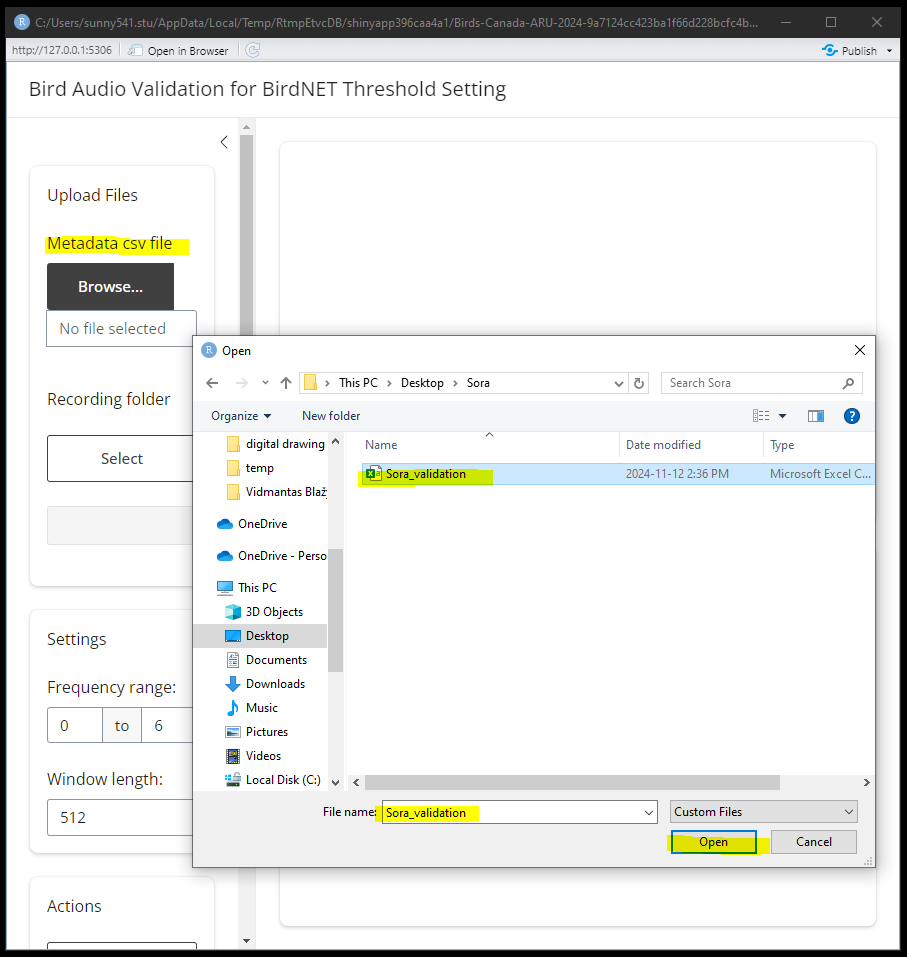
\includegraphics{images/clipboard-3018843216.png} &
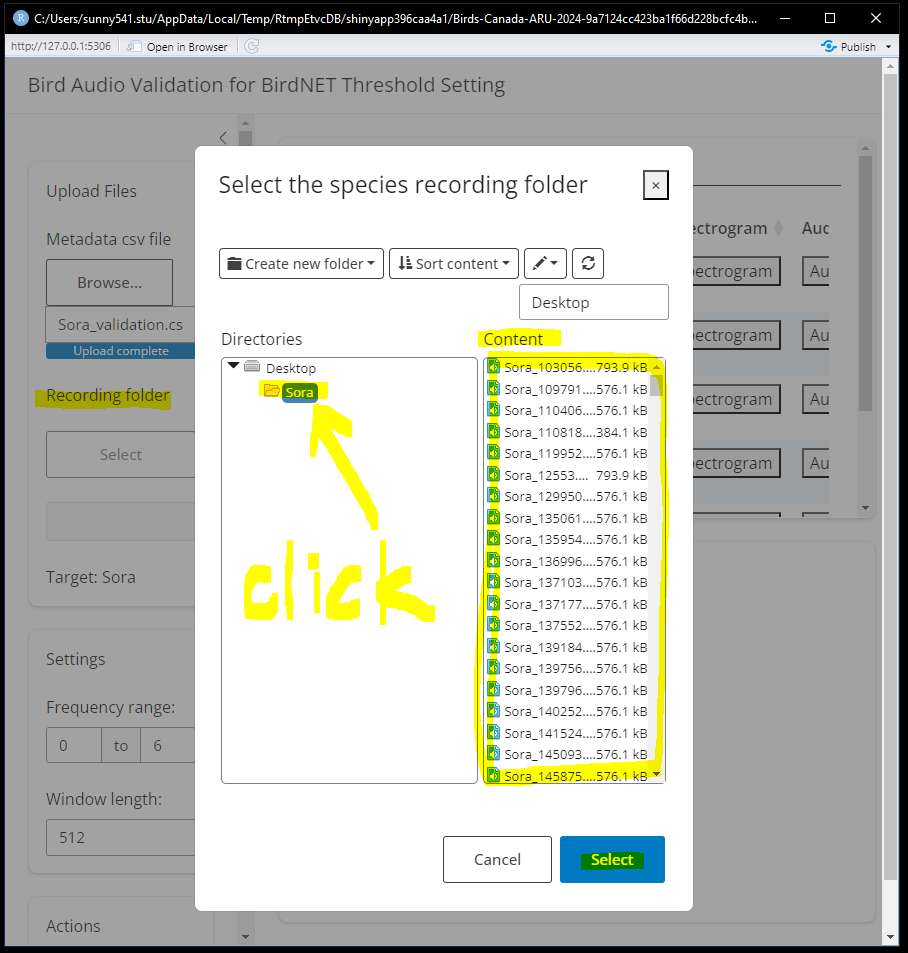
\includegraphics{images/clipboard-1068388884.png} \\
\end{longtable}

\begin{itemize}
\item
  The .csv file would be shown on the top panel (with few selected
  columns). Once you click on the ``Spectrogram'' button, the bottom
  panel would show the corresponded spectrogram. And if you click the
  ``Audio'' button, it would play that specific segment for you.
\item
  You can adjust the ``Settings'' on the left panel to view the
  spectrogram. Click on the ``Praise me'' button if you are feeling
  tired of validating sounds. 😃
\end{itemize}

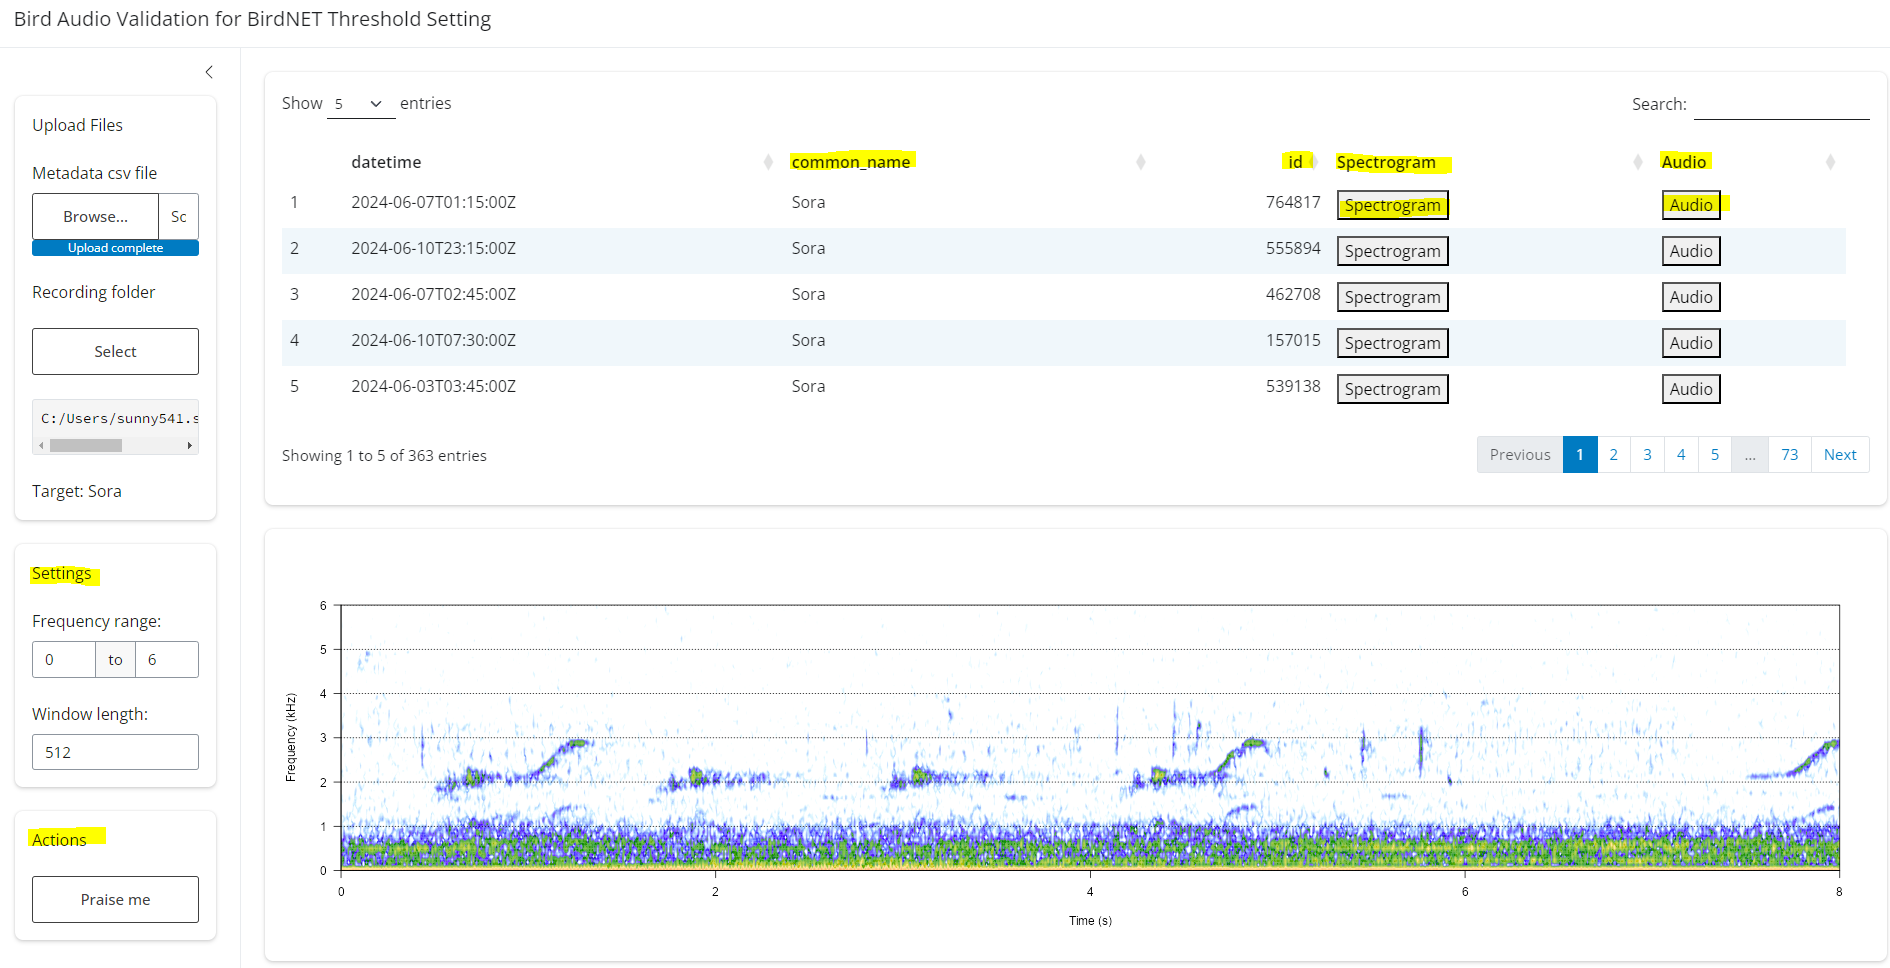
\includegraphics{images/clipboard-2147672079.png}

\subsubsection{Wrap up}\label{wrap-up}

\begin{itemize}
\tightlist
\item
  After completing all the segments, save your file as
  ``SPECIES\_NAME\_validation\_YOUR\_INITIAL.csv''. Upload this .csv
  file to the same folder, or send the final document back to Sunny.
\end{itemize}

\subsubsection{Enjoy!!}\label{enjoy}

\end{document}
